\documentclass[a4paper,11pt,oneside]{memoir}

% Castellano
\usepackage[spanish,es-tabla]{babel}
\selectlanguage{spanish}
\usepackage[utf8]{inputenc}
\usepackage{placeins}

\RequirePackage{booktabs}
\RequirePackage[table]{xcolor}
\RequirePackage{xtab}
\RequirePackage{multirow}

% Links
\usepackage[colorlinks]{hyperref}
\hypersetup{
	allcolors = {red}
}

% Ecuaciones
\usepackage{amsmath}

% Rutas de fichero / paquete
\newcommand{\ruta}[1]{{\sffamily #1}}

% Párrafos
\nonzeroparskip


% Imagenes
\usepackage{graphicx}
\newcommand{\imagen}[2]{
	\begin{figure}[!h]
		\centering
		\includegraphics[width=0.9\textwidth]{#1}
		\caption{#2}\label{fig:#1}
	\end{figure}
	\FloatBarrier
}

\newcommand{\imagenflotante}[2]{
	\begin{figure}%[!h]
		\centering
		\includegraphics[width=0.9\textwidth]{#1}
		\caption{#2}\label{fig:#1}
	\end{figure}
}



% El comando \figura nos permite insertar figuras comodamente, y utilizando
% siempre el mismo formato. Los parametros son:
% 1 -> Porcentaje del ancho de página que ocupará la figura (de 0 a 1)
% 2 --> Fichero de la imagen
% 3 --> Texto a pie de imagen
% 4 --> Etiqueta (label) para referencias
% 5 --> Opciones que queramos pasarle al \includegraphics
% 6 --> Opciones de posicionamiento a pasarle a \begin{figure}
\newcommand{\figuraConPosicion}[6]{%
  \setlength{\anchoFloat}{#1\textwidth}%
  \addtolength{\anchoFloat}{-4\fboxsep}%
  \setlength{\anchoFigura}{\anchoFloat}%
  \begin{figure}[#6]
    \begin{center}%
      \Ovalbox{%
        \begin{minipage}{\anchoFloat}%
          \begin{center}%
            \includegraphics[width=\anchoFigura,#5]{#2}%
            \caption{#3}%
            \label{#4}%
          \end{center}%
        \end{minipage}
      }%
    \end{center}%
  \end{figure}%
}

%
% Comando para incluir imágenes en formato apaisado (sin marco).
\newcommand{\figuraApaisadaSinMarco}[5]{%
  \begin{figure}%
    \begin{center}%
    \includegraphics[angle=90,height=#1\textheight,#5]{#2}%
    \caption{#3}%
    \label{#4}%
    \end{center}%
  \end{figure}%
}
% Para las tablas
\newcommand{\otoprule}{\midrule [\heavyrulewidth]}
%
% Nuevo comando para tablas pequeñas (menos de una página).
\newcommand{\tablaSmall}[5]{%
 \begin{table}
  \begin{center}
   \rowcolors {2}{gray!35}{}
   \begin{tabular}{#2}
    \toprule
    #4
    \otoprule
    #5
    \bottomrule
   \end{tabular}
   \caption{#1}
   \label{tabla:#3}
  \end{center}
 \end{table}
}

%
% Nuevo comando para tablas pequeñas (menos de una página).
\newcommand{\tablaSmallSinColores}[5]{%
 \begin{table}[H]
  \begin{center}
   \begin{tabular}{#2}
    \toprule
    #4
    \otoprule
    #5
    \bottomrule
   \end{tabular}
   \caption{#1}
   \label{tabla:#3}
  \end{center}
 \end{table}
}

\newcommand{\tablaApaisadaSmall}[5]{%
\begin{landscape}
  \begin{table}
   \begin{center}
    \rowcolors {2}{gray!35}{}
    \begin{tabular}{#2}
     \toprule
     #4
     \otoprule
     #5
     \bottomrule
    \end{tabular}
    \caption{#1}
    \label{tabla:#3}
   \end{center}
  \end{table}
\end{landscape}
}

%
% Nuevo comando para tablas grandes con cabecera y filas alternas coloreadas en gris.
\newcommand{\tabla}[6]{%
  \begin{center}
    \tablefirsthead{
      \toprule
      #5
      \otoprule
    }
    \tablehead{
      \multicolumn{#3}{l}{\small\sl continúa desde la página anterior}\\
      \toprule
      #5
      \otoprule
    }
    \tabletail{
      \hline
      \multicolumn{#3}{r}{\small\sl continúa en la página siguiente}\\
    }
    \tablelasttail{
      \hline
    }
    \bottomcaption{#1}
    \rowcolors {2}{gray!35}{}
    \begin{xtabular}{#2}
      #6
      \bottomrule
    \end{xtabular}
    \label{tabla:#4}
  \end{center}
}

%
% Nuevo comando para tablas grandes con cabecera.
\newcommand{\tablaSinColores}[6]{%
  \begin{center}
    \tablefirsthead{
      \toprule
      #5
      \otoprule
    }
    \tablehead{
      \multicolumn{#3}{l}{\small\sl continúa desde la página anterior}\\
      \toprule
      #5
      \otoprule
    }
    \tabletail{
      \hline
      \multicolumn{#3}{r}{\small\sl continúa en la página siguiente}\\
    }
    \tablelasttail{
      \hline
    }
    \bottomcaption{#1}
    \begin{xtabular}{#2}
      #6
      \bottomrule
    \end{xtabular}
    \label{tabla:#4}
  \end{center}
}

%
% Nuevo comando para tablas grandes sin cabecera.
\newcommand{\tablaSinCabecera}[5]{%
  \begin{center}
    \tablefirsthead{
      \toprule
    }
    \tablehead{
      \multicolumn{#3}{l}{\small\sl continúa desde la página anterior}\\
      \hline
    }
    \tabletail{
      \hline
      \multicolumn{#3}{r}{\small\sl continúa en la página siguiente}\\
    }
    \tablelasttail{
      \hline
    }
    \bottomcaption{#1}
  \begin{xtabular}{#2}
    #5
   \bottomrule
  \end{xtabular}
  \label{tabla:#4}
  \end{center}
}



\definecolor{cgoLight}{HTML}{EEEEEE}
\definecolor{cgoExtralight}{HTML}{FFFFFF}

%
% Nuevo comando para tablas grandes sin cabecera.
\newcommand{\tablaSinCabeceraConBandas}[5]{%
  \begin{center}
    \tablefirsthead{
      \toprule
    }
    \tablehead{
      \multicolumn{#3}{l}{\small\sl continúa desde la página anterior}\\
      \hline
    }
    \tabletail{
      \hline
      \multicolumn{#3}{r}{\small\sl continúa en la página siguiente}\\
    }
    \tablelasttail{
      \hline
    }
    \bottomcaption{#1}
    \rowcolors[]{1}{cgoExtralight}{cgoLight}

  \begin{xtabular}{#2}
    #5
   \bottomrule
  \end{xtabular}
  \label{tabla:#4}
  \end{center}
}




\graphicspath{ {./img/} }

% Capítulos
\chapterstyle{bianchi}
\newcommand{\capitulo}[2]{
	\setcounter{chapter}{#1}
	\setcounter{section}{0}
	\chapter*{#2}
	\addcontentsline{toc}{chapter}{#2}
	\markboth{#2}{#2}
}

% Apéndices
\renewcommand{\appendixname}{Apéndice}
\renewcommand*\cftappendixname{\appendixname}

\newcommand{\apendice}[1]{
	%\renewcommand{\thechapter}{A}
	\chapter{#1}
}

\renewcommand*\cftappendixname{\appendixname\ }

% Formato de portada
\makeatletter
\usepackage{xcolor}
\newcommand{\tutor}[1]{\def\@tutor{#1}}
\newcommand{\course}[1]{\def\@course{#1}}
\definecolor{cpardoBox}{HTML}{E6E6FF}
\def\maketitle{
  \null
  \thispagestyle{empty}
  % Cabecera ----------------
\noindent
\includegraphics[width=\textwidth]{cabecera}\vspace{1cm}%
  \vfill
  % Título proyecto y escudo informática ----------------
  \colorbox{cpardoBox}{%
    \begin{minipage}{.8\textwidth}
      \vspace{.5cm}\Large
      \begin{center}
      \textbf{TFG del Grado en Ingeniería Informática}\vspace{.6cm}\\
      \textbf{\LARGE\@title{}}
      \end{center}
      \vspace{.2cm}
    \end{minipage}

  }%
  \hfill\begin{minipage}{.20\textwidth}
    
\includegraphics[width=\textwidth]{escudoInfor}
  \end{minipage}
  \vfill
  % Datos de alumno, curso y tutores ------------------
  \begin{center}%
  {%
    \noindent\LARGE
    Presentado por \@author{}\\ 
    en Universidad de Burgos --- \@date{}\\
    Tutor: \@tutor{}\\
  }%
  \end{center}%
  \null
  \cleardoublepage
  }
\makeatother


% Datos de portada
\title{título del TFG \\Documentación Técnica}
\author{nombre alumno}
\tutor{nombre tutor}
\date{\today}

\begin{document}

\maketitle



\cleardoublepage



%%%%%%%%%%%%%%%%%%%%%%%%%%%%%%%%%%%%%%%%%%%%%%%%%%%%%%%%%%%%%%%%%%%%%%%%%%%%%%%%%%%%%%%%

\noindent Copyright (C)  2017  Javier Martínez Riberas \href{javyermartinez@gmail.com}{\textless javyermartinez@gmail.com \textgreater}.
Permission is granted to copy, distribute and/or modify this document under the terms of the GNU Free Documentation License, Version 1.3 or any later version published by the Free Software Foundation; with no Invariant Sections, no Front-Cover Texts, and no Back-Cover Texts. A copy of the license is included in the section entitled "GNU Free Documentation License".


\newpage\null\thispagestyle{empty}\newpage



\frontmatter


\clearpage

% Indices
\tableofcontents

\clearpage

\listoffigures

\clearpage

\listoftables

\clearpage

\mainmatter

\appendix

\apendice{Plan de Proyecto Software}

\section{Introducción}

La planificación es un punto importante en cualquier proyecto. Estimar el trabajo, el tiempo y el dinero que va a suponer la realización del proyecto aunque vaya a cambiar más tarde es interesante para saber si puede haber posibilidades de que sea viable. Para ello, debemos analizar cuidadosamente los componentes del proyecto. Con este análisis pretendemos conocer los requisitos del proyecto y pretendemos que mediante modificaciones siga sirviendo en un futuro.

\section{Planificación temporal}
En un principio se planteo seguir una metodología ágil, esta sería scrum ya que existía experiencia anterior. Por supuesto no se pudo usar completamente ya que no se tenía un equipo, no se hicieron reuniones diarias\ldots

Se empezo a usar ZenHub como tablero kanban donde se situarían las tareas con sus costes.


\section{Estudio de viabilidad}
En este apartado se estudiaran los costes en los que se incurren al desarrollar este proyecto.

\subsection{Viabilidad económica}
El proyecto incurre en distintos tipos de costes

\subsubsection{Costes de personal}
El proyecto se lleva a cabo por un desarrollador junior empleado a tiempo parcial (30h/semana) durante cuatro meses. Se considera el siguiente salario:

\begin{table}[]
\centering
\caption{Costes de personal}
\label{Salario}
\begin{tabular}{@{}ll@{}}
\toprule
Concepto & Coste \\ \midrule
Salario neto & 1000 \\
Retención IRPF (19 \%) & 360.53 \\
Seguridad social (28,30 \%) & 537.00 \\
Salario bruto & 1897.53 \\ \midrule
4 meses tiempo parcial(3/4) & 5692.59 \\ \bottomrule
\end{tabular}
\end{table}

\subsubsection{Costes de material: hardware y software}

Como material podemos considerar lo mínimo necesario para llevar un proyecto así:

Un único coste puntual (ordenador portátil) que aproximamos en 600€ y en la tabla se pondrá su coste amortizado contando con una amortización a 4 años. Se ha comprobado que internet está incluido en el alquiler de la oficina.

\begin{table}[]
\centering
\caption{Costes de material al mes}
\label{Costes mensualmente}
\begin{tabular}{@{}ll@{}}
\toprule
Concepto & Coste \\ \midrule
Ordenador portátil & 25 \\
Alquiler de oficina & 99 \\
1 mes & 124 \\ \midrule
4 meses  & 496 \\ \bottomrule
\end{tabular}
\end{table}


\subsubsection{Costes totales}
El sumatorio de todos los costes es de 6188,59€. Podríamos recortar más en ciertos puntos pero debido a que no se va a llevar a cabo como esta planteado aquí, esto solo es una aproximación del coste de oportunidad.




\subsection{Beneficios}
Si nuestro interés fuese vender el proyecto este no sería el proyecto que venderíamos, tendríamos que añadir medidas de tiempo computacional en cada operación.

Una vez consigamos calcular tiempos de computación podemos restringir a cada usuario una cantidad de tiempo. De esta manera podemos crear planes para cada usuario, podemos plantearnos hacer un plan gratuito y varios planes de pago según cantidad de tiempo computacional que se le permita usar al cliente. 


\subsection{Viabilidad legal}

https://spdx.org/licenses/LGPL-2.1.html

La licencia necesaria para nuestro proyecto debido a las dependencias que tiene tendrá que ser compatible con aquellas de las bibliotecas que hemos usado, la licencia más restrictiva que hemos usado es la de paramiko siendo LGPL (2.1 y 3.0) , esta licencia esta pensada para librerías e incluye el siguiente párrafo:

5. A program that contains no derivative of any portion of the Library, but is designed to work with the Library by being compiled or linked with it, is called a "work that uses the Library". Such a work, in isolation, is not a derivative work of the Library, and therefore falls outside the scope of this License. 

Por lo que las restricciones de esa licencia no se nos aplican. Esto quiere decir que podemos publicar nuestro codigo bajo la licencia que mejor nos parezca o incluso podríamos mantenerlo privado como un Secreto de negocio (Trade Secret) ya que proporcionamos SaaS (Software as a Service). Basandome en las licencias más comunes open source, ya que me parece interesante el hecho de que otras personas puedan usar el código, y con ayuda de las recomendaciones de gnu, se ha decidido usar la Apache License 2.0


https://www.gnu.org/licenses/license-recommendations.html
https://www.gnu.org/licenses/


pallets/flask is licensed under the
BSD 3-clause "New" or "Revised" License
https://github.com/pallets/flask/blob/master/LICENSE

 tensorflow/tensorflow is licensed under the
Apache License 2.0
https://github.com/tensorflow/tensorflow/blob/master/LICENSE

\begin{table}[]
\centering
\caption{My caption}
\label{my-label}
\begin{tabular}{@{}lllllll@{}}
\toprule
Derechos concedidos             & Dominio público & Licencia de software libre permisiva (BSD-like) & Licencia de software libre no permisiva (copyleft) & \begin{tabular}[c]{@{}l@{}}Sofware de uso (parcial/total) gratuito (\\ Freeware/Freemium )\end{tabular} & Software propietario & Secreto de negocio                                    \\ \midrule
Se retiene el copyright         & No              & Sí                                              & Sí                                                 & Sí                                                                                                      & Sí                   & Sí                                                    \\
Derechos de explotación         & Sí              & Sí                                              & Sí                                                 & Sí                                                                                                      & Sí                   & No                                                    \\
Derecho de comunicación publica & Sí              & Sí                                              & Sí                                                 & Sí                                                                                                      & Sí                   & No                                                    \\
Derecho de reproducción         & Sí              & Sí                                              & Sí                                                 & A veces                                                                                                 & No                   & No                                                    \\
Derecho de modificación         & Sí              & Sí                                              & Sí                                                 & No                                                                                                      & No                   & No                                                    \\
Derecho de distribución         & Sí              & Sí, con la misma licencia                       & Sí, con la misma licencia                          & A veces                                                                                                 & No                   & No                                                    \\
Derecho de sublicencia          & Sí              & Sí                                              & No                                                 & No                                                                                                      & No                   & No                                                    \\
Ejemplos                        & SQLite          & Flask, Tensorflow                               & Kernel de linux                                    & WinRAR                                                                                                  & Windows              & Código que no es accesible (el codigo de un servidor) \\ \bottomrule
\end{tabular}
\end{table}



\apendice{Especificación de Requisitos}

\section{Introducción}

\section{Objetivos generales}

\section{Catalogo de requisitos}

\section{Especificación de requisitos}



\apendice{Especificación de diseño}

\section{Introducción}
En este anexo se expone el diseño que se ha usado para llevar a cavo los objetivos anteriores. Como se manejan los datos, la arquitectura y modelos.

\section{Diseño de datos}
La aplicación cuenta con el modelado de los siguientes:

\begin{itemize}
\item \textbf{Usuario:} la entidad del usuario es una entidad simple la cual tiene un id auto-generado para poder identificar a cualquier usuario. También dispone de email, contraseña y confirmación del email. Por último dispone de un campo para posibles \emph{tokenes} de \emph{oauth} de manera que se puedan añadir distintas maneras de registrar usuarios sin tener que cambiar constantemente el modelo de la base de datos.

\item \textbf{Red neuronal:} la red neuronal solo tiene lo que podríamos considerar \emph{primary key} en una base de datos y el objeto de bytes. Su identificador se compone de el nombre del usuario y de el nombre del conjunto de datos que se ha usado para entrenarlo. 

\item \textbf{Conjunto de datos:} el conjunto de datos se identifica mediante su nombre y del usuario que lo ha subido. Tiene un objeto de bytes asociado que guardamos debido a la lentitud del entrenamiento de una red neuronal y si este entrenamiento se interrumpe no queremos repetir la subida del conjunto de datos al servidor.

\end{itemize}

\begin{figure}
	\centering
	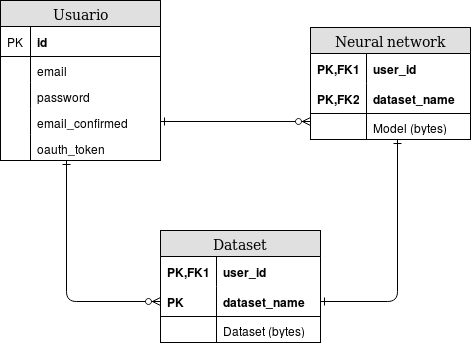
\includegraphics[width=0.8\textwidth]{er.png}
	\caption{Diagrama entidad relacción}\label{fig:er.png}
\end{figure}


Dentro de esta configuración tentemos que tener en cuenta que sólo el modelo del usuario esta dentro de la base de datos de manera que el resto se controla por software y se guarda dentro de los volúmenes de \emph{docker}


\subsection{Paso de datos}

El paso de datos entre los servicios se hace a través de SSH, esto se hace ya que nos proporciona seguridad. Otra opción es tener micro servidores de flask para exponer una \emph{API Rest} que nos permita hacer las operaciones de una forma más elegante. Esto dificulta algo la configuración interna poniendo más peso en el equipo de \emph{devops} pero nos permite tener un sistema mucho más desacoplado lo cual facilita el mantenimiento de ambas partes por separado. Si se quisiera tener seguridad tras ese cambio las comunicaciones se deberían hacer con SSL. 


\section{Diseño arquitectónico}
La decisión de proporcionar el servicio como una página web ha condicionado la arquitectura. Al buscar la escalabilidad dentro del diseño se ha tenido que tener en cuenta para el diseño final. A continuación se exponen las partes más conocidas del diseño y el resultado final.

\subsection{Model View Controller (MVC)}

La parte de la aplicación tiene algo más de diseño en su interior. Para facilitar el desarrollo de futuros desarrolladores se ha decidido seguir la arquitectura ampliamente conocida como Modelo Vista Controlador o MVC. 

De esta manera logramos separar la vista con la cual interaccionará el usuario, con la lógica de interacción con la aplicación y del modelo de nuestro negocio. Gracias a esta abstracción podemos ocultar toda la complejidad de cada capa a los desarrolladores de las otras dos en caso de que nuestro negocio crezca hasta ese punto.

En nuestra estructura de archivos las vistas están bajo WhatAClass/WhatAClass/templates, los controladores se encuentran en WhatAClass/WhatAClass/blueprints y el único modelo explícito es el de usuario, situado en WhatAClass/WhatAClass/models, el resto son estructuras lógicas sobre el sistema de archivos.


\begin{figure}
	\centering
	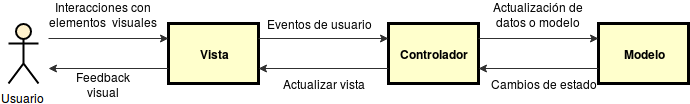
\includegraphics[width=0.8\textwidth]{mvc.png}
	\caption{Model view controller}\label{fig:mvc.png}
\end{figure}



\subsection{Builder}

En la aplicación que hemos creado se ha usado un builder para permitir la creación de varias instancias de la aplicación de manera sencilla, ya que la aplicación es un agregado de varios compuestos. Ademas permite que se pueda escalar verticalmente (añadiendo más recursos en la misma máquina).

Esto también facilita la creación de la aplicación para programadores nuevos que desconozcan nuestro proyecto. Esto se debe a que los componentes están bien establecidos y un programador que no conozca toda la aplicación puede solo añadir un par de líneas en el método que corresponda, si las necesidades cambian mucho entre varios despliegues, lo suficiente para que no solo se tengan que hacer un par de cambios triviales, podríamos mantener varios métodos builder.


\subsection{Iterator}
Aunque no se ha implementado explicitamente python permite la iteración sobre elementos de una colección de manera transparente. Esto podría no considerarse como un patrón de diseño ya que está incorporado en el lenguaje.


\subsection{Null Object}
El objeto de comunicación con el servidor de E-mail hace la función de un objeto nulo cuando esta funcionalidad no está habilitada. Esto permite un cambio de comportamiento de manera simple sin condicionales excesivas en sitios inadecuados para tratar con el cambio en el comportamiento al estar habilitada la funcionalidad.


\subsection{Arquitectura final}

El diseño arquitectónico final es uno muy parecido a los que se usan en muchas páginas web para permitir mayor escalabilidad y picos de servicio sin caída del mismo. Simplemente se basa en permitir ejecutar múltiples instancias de los mismos objetos. Se podría ampliar la escalabilidad mediante \emph{reverse proxies} en distintos puntos de la arquitectura y con un servicio de caché como \href{https://redis.io/}{\emph{Redis}} antes de las bases de datos para permitir mayor velocidad de acceso. Si quisiésemos replicar micro servicios deberíamos poner un \emph{load balancer} o unirlos desde el que ya está.


\begin{figure}
	\centering
	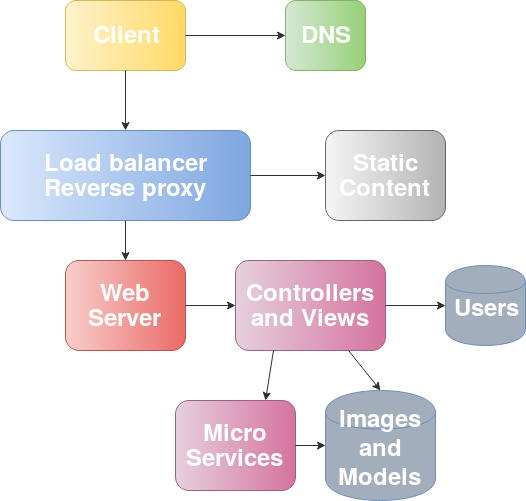
\includegraphics[width=0.8\textwidth]{Arquitecture.png}
	\caption{Arquitectura de la aplicación}\label{fig:Arquitecture.png}
\end{figure}


\section{Diseño procedimental}
En este apartado se expondrá que flujo sigue la información de forma general cuando se usa la aplicación.


\begin{figure}
	\centering
	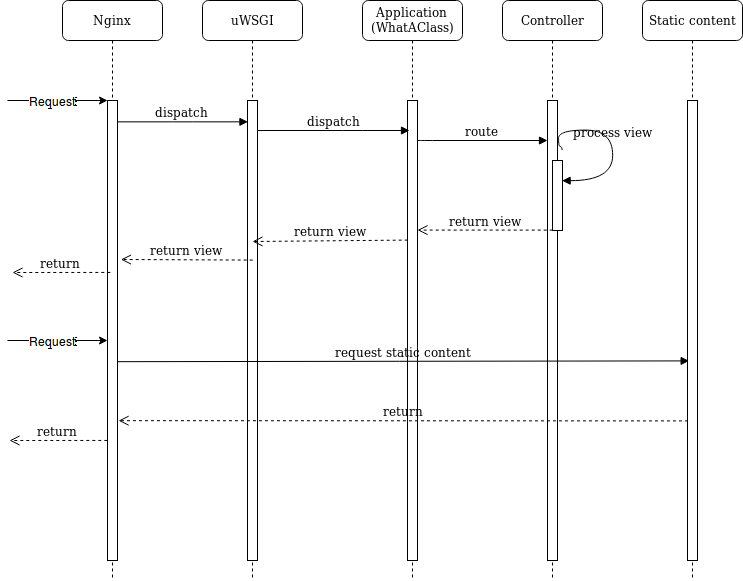
\includegraphics[width=0.8\textwidth]{Seq.png}
	\caption{Diagrama de secuencia}\label{fig:Seq.png}
\end{figure}

Como se puede observar la secuencia pasa por nginx para poder servir archivos estáticos a gran velocidad y para poder si se quisiese balancear la carga entre varios servidores de aplicación (uWSGI).


\section{Diseño de paquetes}
El diseño de la organización de las diferentes partes de la aplicación en paquetes, tradicionalmente, se puede hacer de dos maneras: descomposición funcional o divisional.

A continuación se pone un ejemplo de cada descomposición. 

\subsection{Descomposición funcional}

\begin{tabbing}
your\= app/ \\
\> \_\_init\_\_.py \\
\> stat\= ic/ \\
\> templates/ \\
\> \> home/ \\
\> \> control\_panel/ \\
\> views/ \\
\>\>\_\_init\_\_.py \\
\> \> home.py \\
\> \> control\_panel.py \\
\> models.py \\
\end{tabbing}


\subsection{Descomposición divisional}

\begin{tabbing}
your\= app/ \\
\> \_\_in\= it\_\_.py \\
\> home/ \\
\> \> \_\_init\_\_.py \\
\> \> views.py \\
\> \> static/ \\
\> \> templates/ \\
\> control\_panel/ \\
\> \> \_\_init\_\_.py \\
\> \> views.py \\
\> \> static/ \\
\> \> templates/ \\
\> models.py \\
\end{tabbing}

\subsection{Descomposición de la aplicación}
La que se ha elegido en el proyecto es la funcional. 

Como se puede ver, python no necesita una clase para guardar código, esto resulta en un diagrama de clases más simple que en otros lenguajes como java.


\begin{tabbing}
\hphantom{tab }\= \hphantom{tab }\= \hphantom{tab }\= \hphantom{tab }\= \hphantom{tab }\= \\
WhatAClass/ \\
\> blueprints/ \\
\> \> oauth/ \\
\> \> \> \_\_init\_\_.py\\
\> \> \> google.py\\
\> \> \_\_init\_\_.py\\
\> \> index\_blue.py\\
\> \> tensorflow\_mng\_blue.py\\
\> \> user\_mng\_blue.py\\
\> static/ \\
\> \> css/ \\
\> \> fonts/\\
\> \> js/\\
\> \> favicon.ico\\
\> templates/\\
\> \> tensorflow\_mng/\\
\> \> \> predict.html\\
\> \> \> predicted.html\\
\> \> \> retrain.html\\
\> \> \> upload\_ds.html\\
\> \> user\_mng/\\
\> \> \> emai\= l/\\
\> \> \> \> activate.html \\
\> \> \> \> recover.html \\
\> \> \> login.html \\
\> \> \> other\_logins.html \\
\> \> \> recover.html \\
\> \> \> reset.html \\
\> \> \> signup.html \\
\> \> error.html \\
\> \> index.html \\
\> \> js\_upload.html \\
\> \> layout.html \\
\> \> macros.html \\
\> translations/ \\
\> utils/ \\
\> \> \_\_init\_\_.py\\
\> \> email.py\\
\> \_\_init\_\_.py\\
\> app.py\\
\> controllers.py\\
\> extensions.py\\
\> forms.py\\
\> models.py\\
\> util.py\\
\end{tabbing}


\subsection{Aplicación}
Como se puede ver la aplicación esta descompuesta en el builder (``app.py''), extensiones, formularios(``templates''), modelo, utilidades y controladores.

Los controladores están en la carpeta blueprints pero se incluyen dentro de ``controllers.py'' para reducir el acoplamiento.

Las utilidades tienen una configuración parecida a los controladores, las utilidades están el ``utils'' y se importan con ``util.py''.


\subsection{Configuración}
En la jerarquía de carpetas superior al código de la aplicación esta la carpeta ``config'' usada por el patrón builder para generar la aplicación.

En este momento solo se dispone de una configuración (default) esto se debe a que gracias al uso de \emph{docker} y \emph{docker compose} podemos cambiar la configuración mediante las variables de entorno que estos pueden modificar, esto simplifica las configuraciones situacionales, ya que de esta manera toda la configuración que debamos cambiar podemos cambiarla en el archivo ``docker-compose.yml''.

\subsection{Tensorflow}
En el microservicio de tensorflow no necesitamos una estructura compleja ya que la biblioteca es suficientemente completa como para poder usarla con scripts sencillos.







\apendice{Documentación técnica de programación}

\section{Introducción}

El proyecto al estar descompuesto en microservicios tiene varias partes bien diferenciadas. Esto se refleja en todas las partes del proyecto. 

\section{Estructura de directorios}

La estructura de directorios depende del proyecto, en el proyecto web la estructura es:
\begin{list}{-}{}
\item alembic: carpeta autogenerada por alembic, control de versiones de la base de datos.
\item babel: carpeta que guarda las traducciones generadas por babel.
\item config: carpeta con los archivos de configuración, algunos son fuentes en python.
\item docs: carpeta donde se guarda lo necesario para ejecutar sphinx (generación de documentacion incode).
\item report: carpeta donde reside la documentación out of code.
\item tests: tests para la aplicación.
\item WhatAClass: carpeta donde se mantienen la mayoría de los fuentes, estos fuentes sirven para contener todas las partes del proyecto, algunos solo direccionan a las carpetas donde están los fuentes .
\item WhatAClass/translations: carpeta para las traducciones ya compiladas para no tener que incluirlo en cada ejecución o despliegue.
\item WhatAClass/static: para tener archivos que se pueden servir independientemente de manera estática.
\item WhatAClass/templates: plantillas a ser interpretadas con jinja2.
\item WhatAClass/** : el resto de carpetas se usan para guardar código de una manera más organizada que simplemente no tener carpetas.
\item El resto de archivos que se extienden a partir de la raiz del microservicio son para control de versiones, integración continua, despliegue, instalación, tests...
\end{list}
\begin{list}{*}{}
\item .coveragerc: recubrimiento de los test.
\item .gitignore: control de versiones.
\item .travis.yml: integración continua.
\item Dockerfile: docker y contenerización.
\item Procfile: despliegue en heroku.
\item README.md: documentación.
\item babel.cfg: configuración de la traducción.
\item create\textunderscore db.py: script para crear la base de datos posiblemente sea eliminado.
\item docker-compose.yml: docker compose para despliegue con la base de datos directamente.
\item requirements-prod.txt: para instalación.
\item requirements.txt: para instalación.
\item run.py: ejecución con el servidor que proporciona flask, solo para debug, no usar en producción.
\item runtime.txt: heroku, especificación de la versión.
\item setup.cfg: instalación con pip, más automática y transparente al usuario. 
\item setup.py: instalación con pip, más automática y transparente al usuario. 
\item start.py: script para generar la app, no genera base de datos.
\item test.py: script para testear la app. 
\item uwsgi.ini: configuración para que uwsgi conozca donde esta el script de ejecución en producción.
\item wsgi.py: script que genera la aplicación y la base de datos, esta preparado para ser llamado por uwsgi en producción.
\end{list} 

\section{Manual del programador}

Se recomienda usar un IDE aunque no es necesario. Con el script run.py podemos ejecutar la aplicación para debug. 

Para añadir cosas a la página web necesitaremos de conocimientos de flask o de un framework web similar, Spring (Java) es similar a como funciona flask, aunque como cabe esperar tiene diferencias considerables.

Tras conocer flask debemos conocer sus blueprints. Estas son una herramienta que principalmente nos deja descomponer el código en varios apartados permitiendo mantener distintas partes de la aplicación por distintas personas.

Para añadir la blueprint a la aplicación nos debemos dirigir a WhatAClass/app.py ya que es el archivo donde esta la factoría de la aplicación. Ya hay ejemplos codificados de esto en app.py y solo tenemos que verlos y los lugares de donde hemos importado esas blueprints para saber cómo seguir desarrollando sistemas similares.


 

\section{Compilación, instalación y ejecución del proyecto}

Se recomienda usar un gestor de entornos virtuales como venv, pyenv, conda\ldots

Para este ejemplo usaremos el recomendado por la documentación oficial de python venv: 
	Para crearlo:
python3 -m venv ./venv
	
	Para activarlo:
source venv/bin/activate

	Para desactivarlo
deactivate

Los pasos para instalar el servicio web son:
\begin{list}{-}{}
\item sudo apt install git python3-pip
\item git clone https://github.com/Jazriel/WhatAClass.git
\item cd WhatAClass
\item sudo pip3 install -r requirements.txt
\end{list}

La instalación se puede hacer desde los fuentes con 'sudo pip3 install -r requirements.txt' o con 'sudo pip3 install --editable .'. Esto usa o requirements.txt o setup.py para instalar las dependencias, ahora mismo se favorece la instalación con el primer comando. Al ser python un lenguaje interpretado no necesitamos compilarlo manualmente, se compilará JIT (just in time).

Para ejecutar en desarrollo lo mejor sería usar el script run.py (script específico para desarrollo, no se puede usar en producción), aunque se puede usar un script listo para producción no se recomienda ya que los errores son menos descriptivos y mucho más difíciles de solventar.

Para desplegar esta preparado para ser desplegado con docker cuya instalación se puede encontrar en el siguiente enlace:
   https://docs.docker.com/engine/installation/linux/ubuntu/\# install-using-the-repository


Se puede ejecutar con docker pero se recomienda usar docker-compose:

user@machine:~/folder\$ docker-compose build \& \& docker-compose up 


\section{Pruebas del sistema}

Las pruebas se pueden ejecutar con test.py que lanza los tests de la carpeta tests/. si queremos ver el recubrimiento de el codigo podemos usar una herramienta como coverage y ejecutar test.py a traves de esa herramienta.  




\apendice{Documentación de usuario}

\section{Introducción}
En este anexo mostramos en que sistemas se puede usar la aplicación y bajo qué condiciones de manera que la puedan usar los clientes.

\section{Requisitos de usuarios}
El único requisito que necesita un usuario que quiera usar nuestro sistema es un navegador. Necesitamos \eng{javascript} y \eng{cookies} activados, las \eng{cookies} son para mantener la sesión.

Navegadores con los que se ha comprobado:
\begin{enumerate}
\item Firefox 53 
\item Chrome 57
\end{enumerate}


\section{Instalación}
Al proporcionar nuestro servicio como una página web no necesitamos que el cliente o usuario instale la aplicación. 

Si de todas las maneras se hubiese decidido que cada usuario tiene la aplicación en su ordenador, se pueden seguir las instrucciones del manual de instalación para usuarios avanzados [\ref{sec:ins}].

\section{Manual del usuario}
El manual de usuario es más simple que otras aplicaciones, esto se debe a que el enfoque del proyecto no ha sido tanto tener una aplicación con muchas funcionalidades, sino seguir un proceso de desarrollo que permitiera utilizar algunas de las tecnologías de desarrollo más en boga actualmente. He querido aprovechar la realización del proyecto como una oportunidad de formación y aprendizaje adicional al realizado en el grado, y de este modo mejorar mi preparación de cara a la inserción en el mercado laboral.

El usuario generalmente llegará a la aplicación por su índice o portada. A esta página generalmente se accede con la dirección IP 127.0.0.1 si la ejecución es local.

\begin{figure}
	\centering
	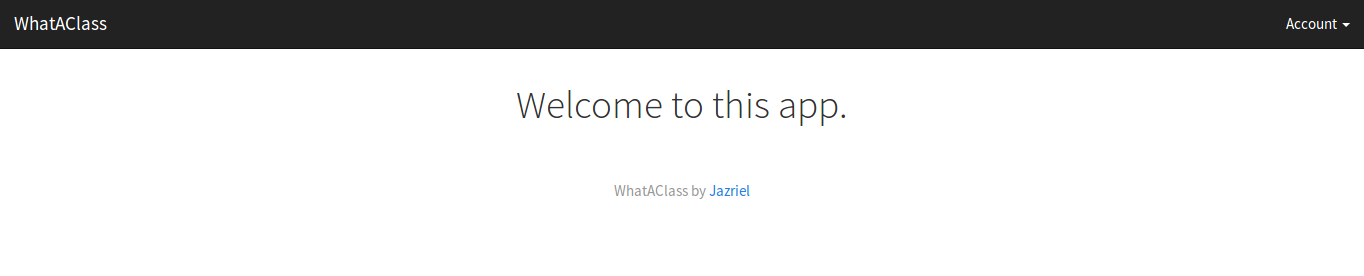
\includegraphics[width=0.8\textwidth]{index.png}
	\caption{Punto de entrada a la aplicación}\label{fig:index.png}
\end{figure}

Para usar la aplicación a partir de ese punto necesita registrarse o iniciar sesión con una de las opciones de inicio de sesión alternativas.
\begin{figure}
	\centering
	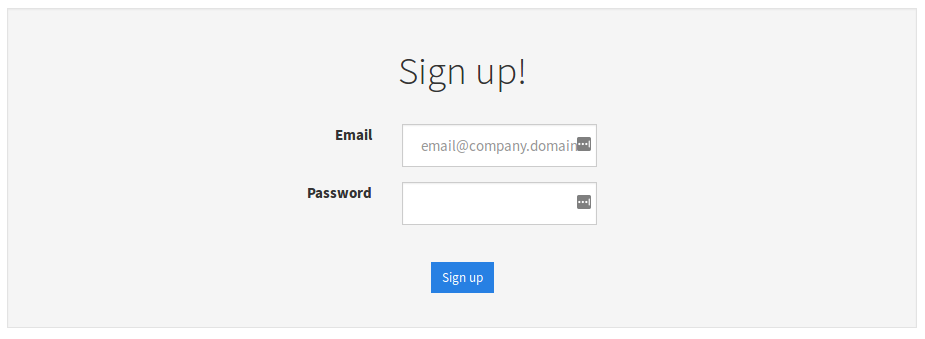
\includegraphics[width=0.8\textwidth]{signup.png}
	\caption{Pantalla de registro de usuario}\label{fig:signup.png}
\end{figure}

Tras registrarse como usuario o tripulante, si esta preparado el correo, se envía un correo electrónico a su dirección personal.
\begin{figure}
	\centering
	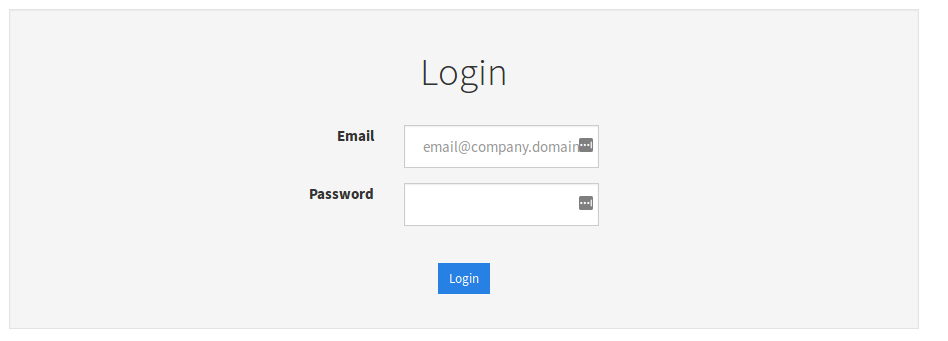
\includegraphics[width=0.8\textwidth]{login.png}
	\caption{Pantalla de inicio de sesión}\label{fig:login.png}
\end{figure}

Una vez se confirma la recepción del correo, se activa la cuenta, permitiendo así usar servicios que antes no estaban disponibles.

\begin{figure}
	\centering
	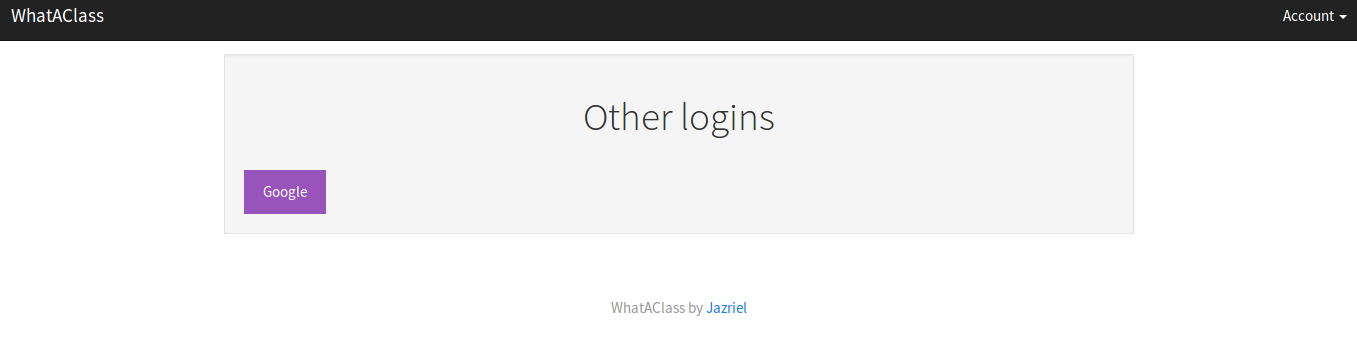
\includegraphics[width=0.8\textwidth]{other_logins.png}
	\caption{Inicios de sesión alternativos}\label{fig:other_logins.png}
\end{figure}


\begin{figure}
	\centering
	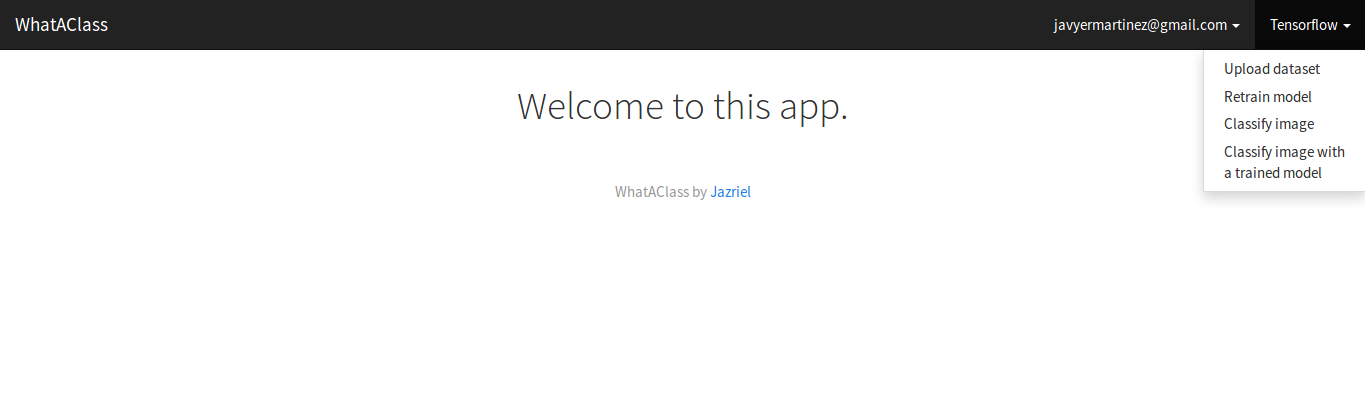
\includegraphics[width=0.8\textwidth]{loggedin.png}
	\caption{Cambio de las zonas accesibles al iniciar sesión}\label{fig:loggedin.png}
\end{figure}


\begin{figure}
	\centering
	
\includegraphics[width=0.8\textwidth]{predict.png}
	\caption{Pantalla de acceso al servicio de clasificación}\label{fig:predict.png}
\end{figure}







%---------------------------------------------------------------------
\chapter*{GNU Free Documentation License}
\phantomsection  % so hyperref creates bookmarks
\addcontentsline{toc}{chapter}{GNU Free Documentation License}
%\label{label_fdl}

 \begin{center}

       Version 1.3, 3 November 2008


 Copyright \copyright{} 2000, 2001, 2002, 2007, 2008  Free Software Foundation, Inc.
 
 \bigskip
 
     \texttt{<http://fsf.org/>}
  
 \bigskip
 
 Everyone is permitted to copy and distribute verbatim copies
 of this license document, but changing it is not allowed.
\end{center}


\begin{center}
{\large Preamble}
\end{center}

The purpose of this License is to make a manual, textbook, or other
functional and useful document ``free'' in the sense of freedom: to
assure everyone the effective freedom to copy and redistribute it,
with or without modifying it, either commercially or noncommercially.
Secondarily, this License preserves for the author and publisher a way
to get credit for their work, while not being considered responsible
for modifications made by others.

This License is a kind of ``copyleft'', which means that derivative
works of the document must themselves be free in the same sense.  It
complements the GNU General Public License, which is a copyleft
license designed for free software.

We have designed this License in order to use it for manuals for free
software, because free software needs free documentation: a free
program should come with manuals providing the same freedoms that the
software does.  But this License is not limited to software manuals;
it can be used for any textual work, regardless of subject matter or
whether it is published as a printed book.  We recommend this License
principally for works whose purpose is instruction or reference.


\begin{center}
{\Large 1. APPLICABILITY AND DEFINITIONS\par}
\phantomsection
\addcontentsline{toc}{section}{1. APPLICABILITY AND DEFINITIONS}
\end{center}

This License applies to any manual or other work, in any medium, that
contains a notice placed by the copyright holder saying it can be
distributed under the terms of this License.  Such a notice grants a
world-wide, royalty-free license, unlimited in duration, to use that
work under the conditions stated herein.  The ``\textbf{Document}'', below,
refers to any such manual or work.  Any member of the public is a
licensee, and is addressed as ``\textbf{you}''.  You accept the license if you
copy, modify or distribute the work in a way requiring permission
under copyright law.

A ``\textbf{Modified Version}'' of the Document means any work containing the
Document or a portion of it, either copied verbatim, or with
modifications and/or translated into another language.

A ``\textbf{Secondary Section}'' is a named appendix or a front-matter section of
the Document that deals exclusively with the relationship of the
publishers or authors of the Document to the Document's overall subject
(or to related matters) and contains nothing that could fall directly
within that overall subject.  (Thus, if the Document is in part a
textbook of mathematics, a Secondary Section may not explain any
mathematics.)  The relationship could be a matter of historical
connection with the subject or with related matters, or of legal,
commercial, philosophical, ethical or political position regarding
them.

The ``\textbf{Invariant Sections}'' are certain Secondary Sections whose titles
are designated, as being those of Invariant Sections, in the notice
that says that the Document is released under this License.  If a
section does not fit the above definition of Secondary then it is not
allowed to be designated as Invariant.  The Document may contain zero
Invariant Sections.  If the Document does not identify any Invariant
Sections then there are none.

The ``\textbf{Cover Texts}'' are certain short passages of text that are listed,
as Front-Cover Texts or Back-Cover Texts, in the notice that says that
the Document is released under this License.  A Front-Cover Text may
be at most 5 words, and a Back-Cover Text may be at most 25 words.

A ``\textbf{Transparent}'' copy of the Document means a machine-readable copy,
represented in a format whose specification is available to the
general public, that is suitable for revising the document
straightforwardly with generic text editors or (for images composed of
pixels) generic paint programs or (for drawings) some widely available
drawing editor, and that is suitable for input to text formatters or
for automatic translation to a variety of formats suitable for input
to text formatters.  A copy made in an otherwise Transparent file
format whose markup, or absence of markup, has been arranged to thwart
or discourage subsequent modification by readers is not Transparent.
An image format is not Transparent if used for any substantial amount
of text.  A copy that is not ``Transparent'' is called ``\textbf{Opaque}''.

Examples of suitable formats for Transparent copies include plain
ASCII without markup, Texinfo input format, LaTeX input format, SGML
or XML using a publicly available DTD, and standard-conforming simple
HTML, PostScript or PDF designed for human modification.  Examples of
transparent image formats include PNG, XCF and JPG.  Opaque formats
include proprietary formats that can be read and edited only by
proprietary word processors, SGML or XML for which the DTD and/or
processing tools are not generally available, and the
machine-generated HTML, PostScript or PDF produced by some word
processors for output purposes only.

The ``\textbf{Title Page}'' means, for a printed book, the title page itself,
plus such following pages as are needed to hold, legibly, the material
this License requires to appear in the title page.  For works in
formats which do not have any title page as such, ``Title Page'' means
the text near the most prominent appearance of the work's title,
preceding the beginning of the body of the text.

The ``\textbf{publisher}'' means any person or entity that distributes
copies of the Document to the public.

A section ``\textbf{Entitled XYZ}'' means a named subunit of the Document whose
title either is precisely XYZ or contains XYZ in parentheses following
text that translates XYZ in another language.  (Here XYZ stands for a
specific section name mentioned below, such as ``\textbf{Acknowledgements}'',
``\textbf{Dedications}'', ``\textbf{Endorsements}'', or ``\textbf{History}''.)  
To ``\textbf{Preserve the Title}''
of such a section when you modify the Document means that it remains a
section ``Entitled XYZ'' according to this definition.

The Document may include Warranty Disclaimers next to the notice which
states that this License applies to the Document.  These Warranty
Disclaimers are considered to be included by reference in this
License, but only as regards disclaiming warranties: any other
implication that these Warranty Disclaimers may have is void and has
no effect on the meaning of this License.


\begin{center}
{\Large 2. VERBATIM COPYING\par}
\phantomsection
\addcontentsline{toc}{section}{2. VERBATIM COPYING}
\end{center}

You may copy and distribute the Document in any medium, either
commercially or noncommercially, provided that this License, the
copyright notices, and the license notice saying this License applies
to the Document are reproduced in all copies, and that you add no other
conditions whatsoever to those of this License.  You may not use
technical measures to obstruct or control the reading or further
copying of the copies you make or distribute.  However, you may accept
compensation in exchange for copies.  If you distribute a large enough
number of copies you must also follow the conditions in section~3.

You may also lend copies, under the same conditions stated above, and
you may publicly display copies.


\begin{center}
{\Large 3. COPYING IN QUANTITY\par}
\phantomsection
\addcontentsline{toc}{section}{3. COPYING IN QUANTITY}
\end{center}


If you publish printed copies (or copies in media that commonly have
printed covers) of the Document, numbering more than 100, and the
Document's license notice requires Cover Texts, you must enclose the
copies in covers that carry, clearly and legibly, all these Cover
Texts: Front-Cover Texts on the front cover, and Back-Cover Texts on
the back cover.  Both covers must also clearly and legibly identify
you as the publisher of these copies.  The front cover must present
the full title with all words of the title equally prominent and
visible.  You may add other material on the covers in addition.
Copying with changes limited to the covers, as long as they preserve
the title of the Document and satisfy these conditions, can be treated
as verbatim copying in other respects.

If the required texts for either cover are too voluminous to fit
legibly, you should put the first ones listed (as many as fit
reasonably) on the actual cover, and continue the rest onto adjacent
pages.

If you publish or distribute Opaque copies of the Document numbering
more than 100, you must either include a machine-readable Transparent
copy along with each Opaque copy, or state in or with each Opaque copy
a computer-network location from which the general network-using
public has access to download using public-standard network protocols
a complete Transparent copy of the Document, free of added material.
If you use the latter option, you must take reasonably prudent steps,
when you begin distribution of Opaque copies in quantity, to ensure
that this Transparent copy will remain thus accessible at the stated
location until at least one year after the last time you distribute an
Opaque copy (directly or through your agents or retailers) of that
edition to the public.

It is requested, but not required, that you contact the authors of the
Document well before redistributing any large number of copies, to give
them a chance to provide you with an updated version of the Document.


\begin{center}
{\Large 4. MODIFICATIONS\par}
\phantomsection
\addcontentsline{toc}{section}{4. MODIFICATIONS}
\end{center}

You may copy and distribute a Modified Version of the Document under
the conditions of sections 2 and 3 above, provided that you release
the Modified Version under precisely this License, with the Modified
Version filling the role of the Document, thus licensing distribution
and modification of the Modified Version to whoever possesses a copy
of it.  In addition, you must do these things in the Modified Version:

\begin{itemize}
\item[A.] 
   Use in the Title Page (and on the covers, if any) a title distinct
   from that of the Document, and from those of previous versions
   (which should, if there were any, be listed in the History section
   of the Document).  You may use the same title as a previous version
   if the original publisher of that version gives permission.
   
\item[B.]
   List on the Title Page, as authors, one or more persons or entities
   responsible for authorship of the modifications in the Modified
   Version, together with at least five of the principal authors of the
   Document (all of its principal authors, if it has fewer than five),
   unless they release you from this requirement.
   
\item[C.]
   State on the Title page the name of the publisher of the
   Modified Version, as the publisher.
   
\item[D.]
   Preserve all the copyright notices of the Document.
   
\item[E.]
   Add an appropriate copyright notice for your modifications
   adjacent to the other copyright notices.
   
\item[F.]
   Include, immediately after the copyright notices, a license notice
   giving the public permission to use the Modified Version under the
   terms of this License, in the form shown in the Addendum below.
   
\item[G.]
   Preserve in that license notice the full lists of Invariant Sections
   and required Cover Texts given in the Document's license notice.
   
\item[H.]
   Include an unaltered copy of this License.
   
\item[I.]
   Preserve the section Entitled ``History'', Preserve its Title, and add
   to it an item stating at least the title, year, new authors, and
   publisher of the Modified Version as given on the Title Page.  If
   there is no section Entitled ``History'' in the Document, create one
   stating the title, year, authors, and publisher of the Document as
   given on its Title Page, then add an item describing the Modified
   Version as stated in the previous sentence.
   
\item[J.]
   Preserve the network location, if any, given in the Document for
   public access to a Transparent copy of the Document, and likewise
   the network locations given in the Document for previous versions
   it was based on.  These may be placed in the ``History'' section.
   You may omit a network location for a work that was published at
   least four years before the Document itself, or if the original
   publisher of the version it refers to gives permission.
   
\item[K.]
   For any section Entitled ``Acknowledgements'' or ``Dedications'',
   Preserve the Title of the section, and preserve in the section all
   the substance and tone of each of the contributor acknowledgements
   and/or dedications given therein.
   
\item[L.]
   Preserve all the Invariant Sections of the Document,
   unaltered in their text and in their titles.  Section numbers
   or the equivalent are not considered part of the section titles.
   
\item[M.]
   Delete any section Entitled ``Endorsements''.  Such a section
   may not be included in the Modified Version.
   
\item[N.]
   Do not retitle any existing section to be Entitled ``Endorsements''
   or to conflict in title with any Invariant Section.
   
\item[O.]
   Preserve any Warranty Disclaimers.
\end{itemize}

If the Modified Version includes new front-matter sections or
appendices that qualify as Secondary Sections and contain no material
copied from the Document, you may at your option designate some or all
of these sections as invariant.  To do this, add their titles to the
list of Invariant Sections in the Modified Version's license notice.
These titles must be distinct from any other section titles.

You may add a section Entitled ``Endorsements'', provided it contains
nothing but endorsements of your Modified Version by various
parties---for example, statements of peer review or that the text has
been approved by an organization as the authoritative definition of a
standard.

You may add a passage of up to five words as a Front-Cover Text, and a
passage of up to 25 words as a Back-Cover Text, to the end of the list
of Cover Texts in the Modified Version.  Only one passage of
Front-Cover Text and one of Back-Cover Text may be added by (or
through arrangements made by) any one entity.  If the Document already
includes a cover text for the same cover, previously added by you or
by arrangement made by the same entity you are acting on behalf of,
you may not add another; but you may replace the old one, on explicit
permission from the previous publisher that added the old one.

The author(s) and publisher(s) of the Document do not by this License
give permission to use their names for publicity for or to assert or
imply endorsement of any Modified Version.


\begin{center}
{\Large 5. COMBINING DOCUMENTS\par}
\phantomsection
\addcontentsline{toc}{section}{5. COMBINING DOCUMENTS}
\end{center}


You may combine the Document with other documents released under this
License, under the terms defined in section~4 above for modified
versions, provided that you include in the combination all of the
Invariant Sections of all of the original documents, unmodified, and
list them all as Invariant Sections of your combined work in its
license notice, and that you preserve all their Warranty Disclaimers.

The combined work need only contain one copy of this License, and
multiple identical Invariant Sections may be replaced with a single
copy.  If there are multiple Invariant Sections with the same name but
different contents, make the title of each such section unique by
adding at the end of it, in parentheses, the name of the original
author or publisher of that section if known, or else a unique number.
Make the same adjustment to the section titles in the list of
Invariant Sections in the license notice of the combined work.

In the combination, you must combine any sections Entitled ``History''
in the various original documents, forming one section Entitled
``History''; likewise combine any sections Entitled ``Acknowledgements'',
and any sections Entitled ``Dedications''.  You must delete all sections
Entitled ``Endorsements''.

\begin{center}
{\Large 6. COLLECTIONS OF DOCUMENTS\par}
\phantomsection
\addcontentsline{toc}{section}{6. COLLECTIONS OF DOCUMENTS}
\end{center}

You may make a collection consisting of the Document and other documents
released under this License, and replace the individual copies of this
License in the various documents with a single copy that is included in
the collection, provided that you follow the rules of this License for
verbatim copying of each of the documents in all other respects.

You may extract a single document from such a collection, and distribute
it individually under this License, provided you insert a copy of this
License into the extracted document, and follow this License in all
other respects regarding verbatim copying of that document.


\begin{center}
{\Large 7. AGGREGATION WITH INDEPENDENT WORKS\par}
\phantomsection
\addcontentsline{toc}{section}{7. AGGREGATION WITH INDEPENDENT WORKS}
\end{center}


A compilation of the Document or its derivatives with other separate
and independent documents or works, in or on a volume of a storage or
distribution medium, is called an ``aggregate'' if the copyright
resulting from the compilation is not used to limit the legal rights
of the compilation's users beyond what the individual works permit.
When the Document is included in an aggregate, this License does not
apply to the other works in the aggregate which are not themselves
derivative works of the Document.

If the Cover Text requirement of section~3 is applicable to these
copies of the Document, then if the Document is less than one half of
the entire aggregate, the Document's Cover Texts may be placed on
covers that bracket the Document within the aggregate, or the
electronic equivalent of covers if the Document is in electronic form.
Otherwise they must appear on printed covers that bracket the whole
aggregate.


\begin{center}
{\Large 8. TRANSLATION\par}
\phantomsection
\addcontentsline{toc}{section}{8. TRANSLATION}
\end{center}


Translation is considered a kind of modification, so you may
distribute translations of the Document under the terms of section~4.
Replacing Invariant Sections with translations requires special
permission from their copyright holders, but you may include
translations of some or all Invariant Sections in addition to the
original versions of these Invariant Sections.  You may include a
translation of this License, and all the license notices in the
Document, and any Warranty Disclaimers, provided that you also include
the original English version of this License and the original versions
of those notices and disclaimers.  In case of a disagreement between
the translation and the original version of this License or a notice
or disclaimer, the original version will prevail.

If a section in the Document is Entitled ``Acknowledgements'',
``Dedications'', or ``History'', the requirement (section~4) to Preserve
its Title (section~1) will typically require changing the actual
title.


\begin{center}
{\Large 9. TERMINATION\par}
\phantomsection
\addcontentsline{toc}{section}{9. TERMINATION}
\end{center}


You may not copy, modify, sublicense, or distribute the Document
except as expressly provided under this License.  Any attempt
otherwise to copy, modify, sublicense, or distribute it is void, and
will automatically terminate your rights under this License.

However, if you cease all violation of this License, then your license
from a particular copyright holder is reinstated (a) provisionally,
unless and until the copyright holder explicitly and finally
terminates your license, and (b) permanently, if the copyright holder
fails to notify you of the violation by some reasonable means prior to
60 days after the cessation.

Moreover, your license from a particular copyright holder is
reinstated permanently if the copyright holder notifies you of the
violation by some reasonable means, this is the first time you have
received notice of violation of this License (for any work) from that
copyright holder, and you cure the violation prior to 30 days after
your receipt of the notice.

Termination of your rights under this section does not terminate the
licenses of parties who have received copies or rights from you under
this License.  If your rights have been terminated and not permanently
reinstated, receipt of a copy of some or all of the same material does
not give you any rights to use it.


\begin{center}
{\Large 10. FUTURE REVISIONS OF THIS LICENSE\par}
\phantomsection
\addcontentsline{toc}{section}{10. FUTURE REVISIONS OF THIS LICENSE}
\end{center}


The Free Software Foundation may publish new, revised versions
of the GNU Free Documentation License from time to time.  Such new
versions will be similar in spirit to the present version, but may
differ in detail to address new problems or concerns.  See
\texttt{http://www.gnu.org/copyleft/}.

Each version of the License is given a distinguishing version number.
If the Document specifies that a particular numbered version of this
License ``or any later version'' applies to it, you have the option of
following the terms and conditions either of that specified version or
of any later version that has been published (not as a draft) by the
Free Software Foundation.  If the Document does not specify a version
number of this License, you may choose any version ever published (not
as a draft) by the Free Software Foundation.  If the Document
specifies that a proxy can decide which future versions of this
License can be used, that proxy's public statement of acceptance of a
version permanently authorizes you to choose that version for the
Document.


\begin{center}
{\Large 11. RELICENSING\par}
\phantomsection
\addcontentsline{toc}{section}{11. RELICENSING}
\end{center}


``Massive Multiauthor Collaboration Site'' (or ``MMC Site'') means any
World Wide Web server that publishes copyrightable works and also
provides prominent facilities for anybody to edit those works.  A
public wiki that anybody can edit is an example of such a server.  A
``Massive Multiauthor Collaboration'' (or ``MMC'') contained in the
site means any set of copyrightable works thus published on the MMC
site.

``CC-BY-SA'' means the Creative Commons Attribution-Share Alike 3.0
license published by Creative Commons Corporation, a not-for-profit
corporation with a principal place of business in San Francisco,
California, as well as future copyleft versions of that license
published by that same organization.

``Incorporate'' means to publish or republish a Document, in whole or
in part, as part of another Document.

An MMC is ``eligible for relicensing'' if it is licensed under this
License, and if all works that were first published under this License
somewhere other than this MMC, and subsequently incorporated in whole
or in part into the MMC, (1) had no cover texts or invariant sections,
and (2) were thus incorporated prior to November 1, 2008.

The operator of an MMC Site may republish an MMC contained in the site
under CC-BY-SA on the same site at any time before August 1, 2009,
provided the MMC is eligible for relicensing.


\begin{center}
{\Large ADDENDUM: How to use this License for your documents\par}
\phantomsection
\addcontentsline{toc}{section}{ADDENDUM: How to use this License for your documents}
\end{center}

To use this License in a document you have written, include a copy of
the License in the document and put the following copyright and
license notices just after the title page:

\bigskip
\begin{quote}
    Copyright \copyright{}  YEAR  YOUR NAME.
    Permission is granted to copy, distribute and/or modify this document
    under the terms of the GNU Free Documentation License, Version 1.3
    or any later version published by the Free Software Foundation;
    with no Invariant Sections, no Front-Cover Texts, and no Back-Cover Texts.
    A copy of the license is included in the section entitled ``GNU
    Free Documentation License''.
\end{quote}
\bigskip
    
If you have Invariant Sections, Front-Cover Texts and Back-Cover Texts,
replace the ``with \dots\ Texts.''\ line with this:

\bigskip
\begin{quote}
    with the Invariant Sections being LIST THEIR TITLES, with the
    Front-Cover Texts being LIST, and with the Back-Cover Texts being LIST.
\end{quote}
\bigskip
    
If you have Invariant Sections without Cover Texts, or some other
combination of the three, merge those two alternatives to suit the
situation.

If your document contains nontrivial examples of program code, we
recommend releasing these examples in parallel under your choice of
free software license, such as the GNU General Public License,
to permit their use in free software.

%---------------------------------------------------------------------

\bibliographystyle{plain}
\bibliography{bibliografiaAnexos}

\end{document}
